\documentclass[tikz,border=0pt]{standalone}
\usepackage[american]{circuitikz}
\usetikzlibrary{arrows.meta,calc,positioning,decorations.pathmorphing,patterns}
\definecolor{zyloTeal}{HTML}{174A5B}
\definecolor{zyloTealTwo}{HTML}{246B7A}
\definecolor{zyloInk}{HTML}{1F2933}
\definecolor{zyloSoft}{HTML}{EAF4F4}
\definecolor{zyloPaper}{HTML}{F8FAFB}
\definecolor{zyloLine}{HTML}{44606B}
\definecolor{zyloOrange}{HTML}{D97706}
\begin{document}
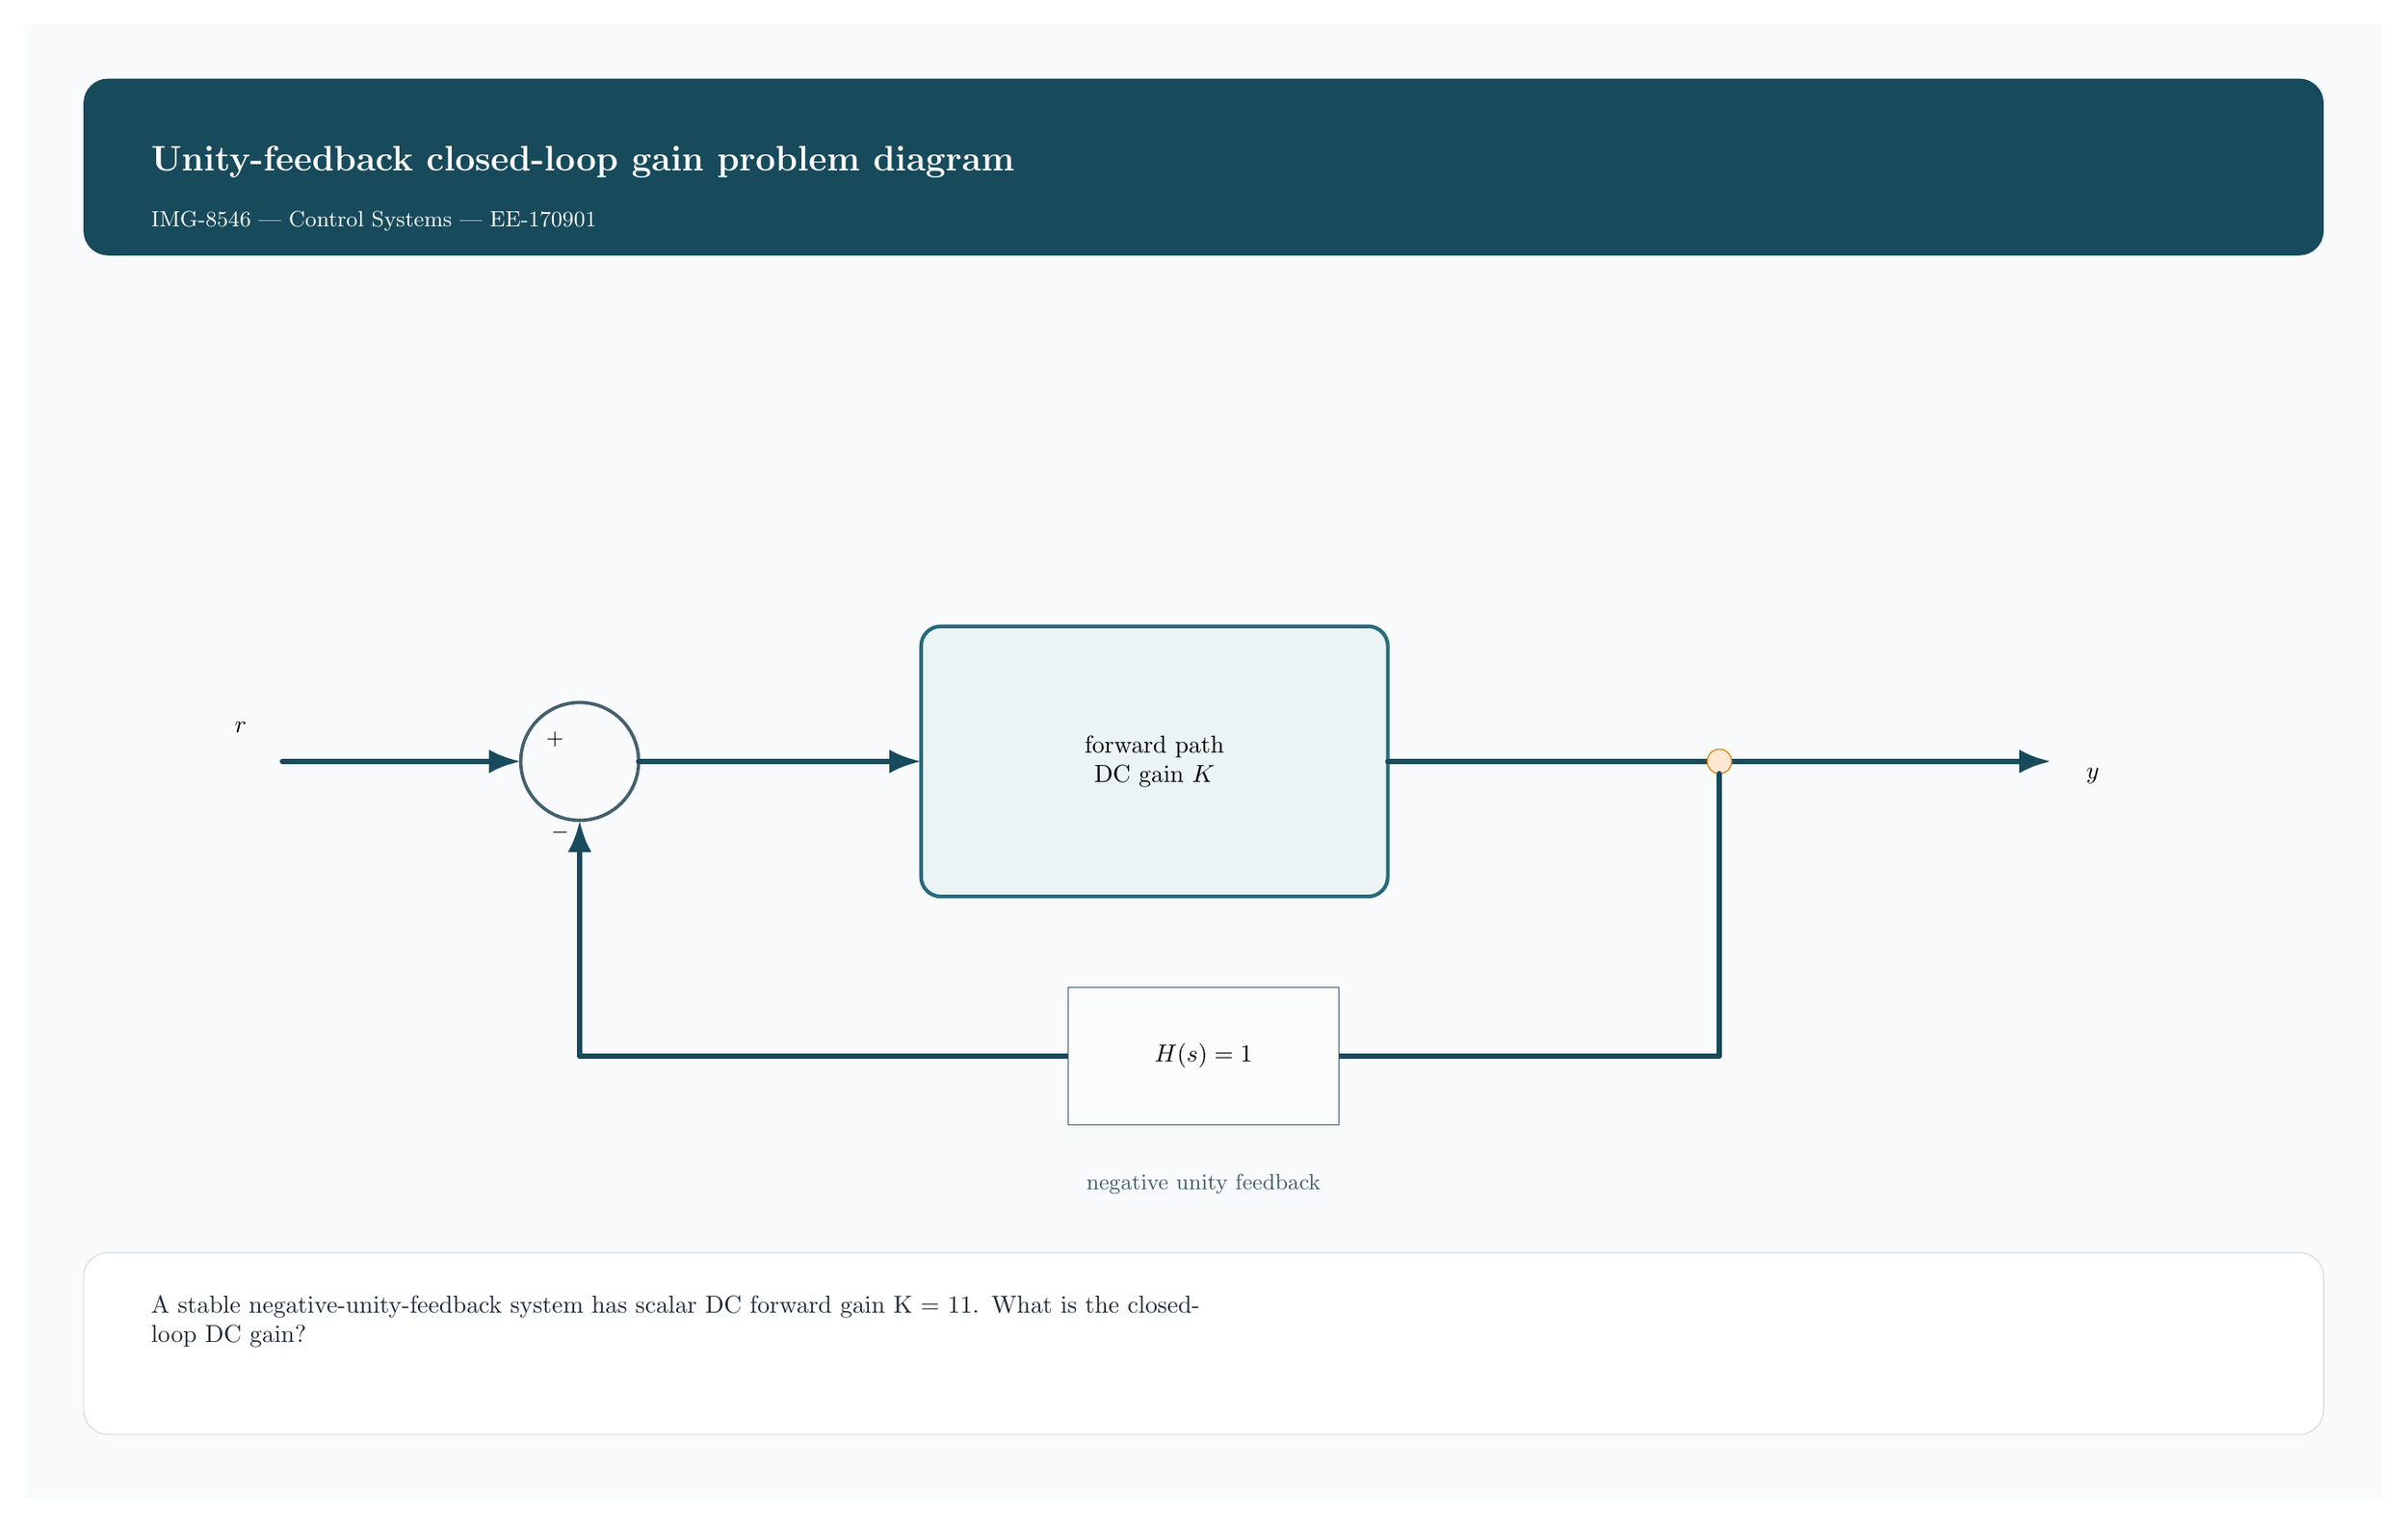
\begin{tikzpicture}[x=1pt,y=-1pt,>=Latex,line cap=round,line join=round]
\path[fill=zyloPaper] (0,0) rectangle (960,600);
\path[fill=zyloTeal,rounded corners=10pt] (24,22) rectangle (936,94);
\node[anchor=west,text=white,font=\bfseries\Large] at (48,56) {Unity-feedback closed-loop gain problem diagram};
\node[anchor=west,text=white!82,font=\small] at (48,80) {IMG-8546 | Control Systems | EE-170901};
\tikzset{wire/.style={draw=zyloTeal,line width=2.2pt},thinwire/.style={draw=zyloLine,line width=1.35pt},accent/.style={draw=zyloOrange,line width=2.2pt},box/.style={draw=zyloTealTwo,fill=zyloSoft,line width=1.5pt,rounded corners=8pt}}
\node at (88,286) {$r$}; \draw[wire,->] (105,300) -- (202,300);
\draw[thinwire] (226,300) circle (24); \node[font=\small] at (216,291) {$+$}; \node[font=\small] at (218,329) {$-$};
\draw[wire,->] (250,300) -- (365,300);
\node[box,minimum width=190pt,minimum height=110pt,align=center] at (460,300) {forward path\\DC gain $K$};
\draw[wire,->] (555,300) -- (825,300); \node at (842,306) {$y$};
\filldraw[draw=zyloOrange,fill=orange!18] (690,300) circle (5);
\draw[wire,->] (690,305) -- (690,420) -- (226,420) -- (226,324);
\node[draw=zyloLine,fill=white!80!zyloSoft,minimum width=110pt,minimum height=56pt] at (480,420) {$H(s)=1$};
\node[font=\small,text=zyloLine] at (480,472) {negative unity feedback};
\path[draw=black!15,fill=white,rounded corners=10pt] (24,500) rectangle (936,574);
\node[anchor=west,text width=860pt,align=left,text=zyloInk,font=\normalsize] at (48,528) {A stable negative-unity-feedback system has scalar DC forward gain K = 11. What is the closed-\\loop DC gain?};
\end{tikzpicture}
\end{document}
